\chapter{Implementation}\label{chap:implementation}
This chapter is dedicated to the description of the implementation details of the particular methods and neural models. We will introduce the architecture of the models, as well as the data pre-processing, training procedures and optimization parameters used.

\section{Deep Depth Pose model}
In this section, we are going to describe our implementation of the DDP model (proposed in \cite{Marin18jvcir}) in Keras framework. The follow-up additional modifications of the model are presented at the end of the section.\par
\vspace{5mm}
\noindent
The DDP model is based on the idea of linearly combining the predefined prototype poses to obtain the resulting pose estimation. The set of prototype poses is produced by clustering the training dataset into $K$ clusters, $K$ being a hyperparameter of the network. The output of the model represents $K$ weights, each corresponding to one of the prototype poses. The final estimated pose is then obtained as a sum of the weighted prototypes.


\subsection{Model structure}

The architecure of the DDP model itself is relatively simple. The model is actually not very deep, it consists of five convolutional blocks, each followed by ReLU activation. First three blocks also contain a pooling layer, as indicated in Fig \ref{fig:ddp}. After the convolutional blocks, there are three fully-connected layers. The number of neurons in the output layer is a hyperparameter set to the number of prototype poses clustered from the dataset. The input to the model is a one-channel depth map of size 100 x 100 pixels.\par

\vspace{5mm}
\begin{figure}[H]
\begin{center}
  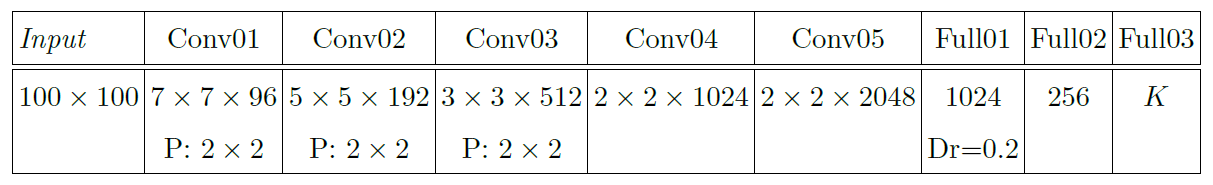
\includegraphics[width=\textwidth]{images/implementation/ddp.PNG}
  \caption[Deep Depth Pose model architecture \cite{Marin18jvcir}.]{Deep Depth Pose model architecture \cite{Marin18jvcir} (\textit{P} stands for pooling layer, \textit{Dr} indicates dropout, $K$ is the number of prototype poses).}
  \label{fig:ddp}
\end{center}
\end{figure}


\subsection{Loss function}

The loss function used during training the model is defined as huber loss with a regularization term, as described in Eq. \ref{eq:huberloss}, where $\mathcal{L}_R$ is the (residual) huber loss.\par

\begin{equation}
\mathcal{L}_{DDP}(g(\mathbf{D}, \theta), \mathbf{C}, \mathbf{p}, \alpha) = (1 - \alpha) \cdot \mathcal{L}_R(\mathbf{C} \times g(\mathbf{D}, \theta), \mathbf{p}) + \alpha \cdot \|g(\mathbf{D}, \theta)\|_1 \label{eq:huberloss}
\end{equation} 

\noindent In the equation above, $g(\mathbf{D}, \theta)$ represents a non-linear function computed by the neural model on the input depth map $\mathbf{D}$ with trainable parameters $\theta$, returning a column vector of length $K$ (number of clustered prototype poses), $\mathbf{C}$ is a matrix with $K$ columns containing prototype poses, $\mathbf{p}$ stands for the vectorized ground-truth pose,  and $\alpha$ is a regularization coefficient  – a hyperparameter to control the magnitude of the resulting weights of the prototypes.

\subsection{Initialization}

The values of the model's hyperparameters from the original DDP paper were chosen using the 'Mann-Whitney U-test' \cite{mann1947}, thus determining, whether the median difference between pairs of configurations are statistically significant. The value of the regularization coefficient was fixed to $\alpha = 0.08$ for the ITOP dataset, and $\alpha = 0.01$ for the UBC3V dataset. The number of prototypes was set to $K=70$ and $K=100$ regarding the ITOP and the UBC3V dataset respectively.\par
\vspace{5mm}
\noindent
The model learns using the Adam optimizer with the learning rate set to $10^{-3}$, which is progressively decreasing during the training.  The weights in the model are initialized using the Xavier normal initializer, that is randomly chosen from the normal distribution with zero mean and a standard deviation proportional to the filter size. The biases are initially set to zero.

\subsection{Data pre-processing}

In the pre-processing stage, the depth maps are re-sized to match the model input dimensions. First, the image is cropped along the larger dimension on both sides to fit the square, assuming the subject is located near the center of the image. Then, the image is re-sized to $100\times100$ px. Afterwards, the depth values are normalized to range [0,1]. Also, the input depth images are normalized globally by subtracting the mean image of the training set from each depth sample. The ground-truth poses are being normalized as well – to zero mean and one standard deviation.\par
\vspace{5mm}
\noindent 
Concerning the datasets used for evaluation, UBC3V already comes with the split into the train, validation and test set. The ITOP dataset is originally divided into the train and test set only, thus the validation set was acquired by random sampling of the train data. The ratio was set to 80/20, meaning the data used for validation are representing 20\% of the train set. During the experiments, only the hard-pose part of UBC3V, and the side-view part (for single-view approach) of the ITOP dataset were used.

%\subsection{Train phase}
%
%\subsection{Test phase}

\subsection{Modifications}
This section introduces several modifications we made to the proposed DDP model, in order to lower the mean error of the predictions. Since the experience of the researchers made us believe that the implementation of the same model in different framework often leads to different results, we diverted from the original architecture of the model, as well as the initial optimization parameters.\par
\vspace{5mm}

\noindent
However, still inspired by the DDP model, we have built a slightly deeper, more complex model, in an attempt to improve the final estimations. We used both ITOP and UBC3V datasets again, for the evaluation of the modified model.
The architecture of the modified DDP network is shown in Fig. \ref{fig:mddp}. As shown in the figure, we significantly increased the amount of drop-out layers, as the model tended to overfit the training data. Moreover, two additional convolutional layers were stacked in the model architecture.\par
\vspace{5mm}

\begin{figure}[H]
\begin{center}
  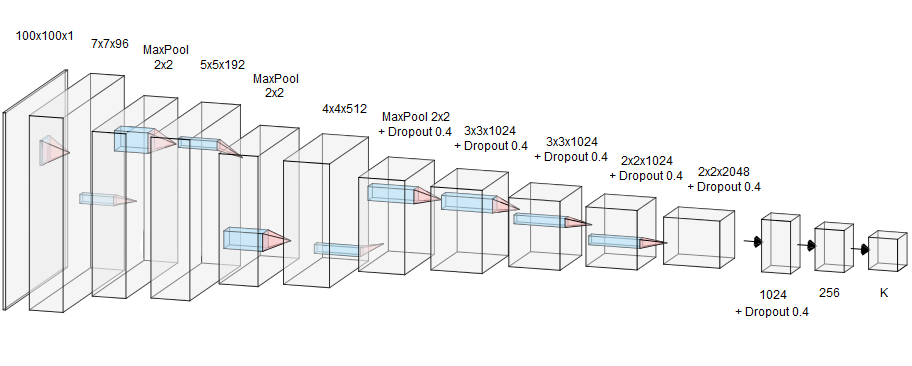
\includegraphics[width=\textwidth]{images/implementation/mddp.png}
  \caption[Our modification of the original DDP model architecture.]{Our modification of the original DDP model architecture\break (\textit{K} stands for the number of prototype poses).}
  \label{fig:mddp}
\end{center}
\end{figure}


\noindent Besides the structure of the model, some of the hyperparameters were slightly modified as well, mainly due to switching to another deep learning framework, where the back-end procedures differ, which may be resulting in a convergence to different outputs. The regularization parameter was fixed to $\alpha = 0.1$ for both benchmark datasets. The residual huber loss was replaced by an absolute error, and the L2 norm was used in the regularization term instead of the L1 norm. Also, the initial learning rate was reduced to $10^{-4}$.\par
\vspace{5mm}
\noindent Regarding the test phase, the experiments on the ITOP dataset have shown that even though the test set seems sufficiently representative (that is, retains the approximate distribution of the training set), the error on the test data is by far worse than the error on previously unseen data obtained by random sampling of the training set (used as a validation set). This is probably caused by the fact, that the input data is formed by a sequence of video frames, thus many subsequent samples captures almost the same content, with only a minimal shift between the frames. As a result, a lot of the validation samples are nearly the same as the ones used for training.\par
\vspace{5mm}
\noindent
The final results of both the original DDP and modified DDP model, evaluated on the test set of ITOP and UBC3V datasets, are reported and discussed in Chapter 7.


\section{Point-Based Pose Estimation model}

As another part of our study, we chose to examine the Point-Base Pose Estimation (PBPE) model \cite{Ali19}. Again, we re-implement the method in Keras framework, though the original implementation was in pure Tensorflow. However, note that the original code was not published prior to our implementation.\par
\vspace{5mm}
\noindent % TODO este popisat zakladnu myslienku modelu



\subsection{Model structure}
 % TODO popisat blizsie vrstvy - a hlavne aj shared MLP -jeho funkcia, zmysel, lokalne, glob. priznaky
The architecture of the proposed model consists of two branches (or sub-networks). The auxiliary sub-network is included to compute the body-part segmentation on the fly, while the main network regresses the joint locations. The basic idea behind the structure of the model is the aggregation of both local and global features of the input point cloud in the auxiliary part-segmentation network. Without the sub-network, almost all of the local context would be lost because of the max-pooling aggregation in the intermediate layers. The incorporation of the local features helps the network understand the relationships among particular local regions of the human body. The whole architecture of the stated model is shown in Fig. \ref{fig:PBPE}.\par
\vspace{5mm}

\begin{figure}[H]
\begin{center}
  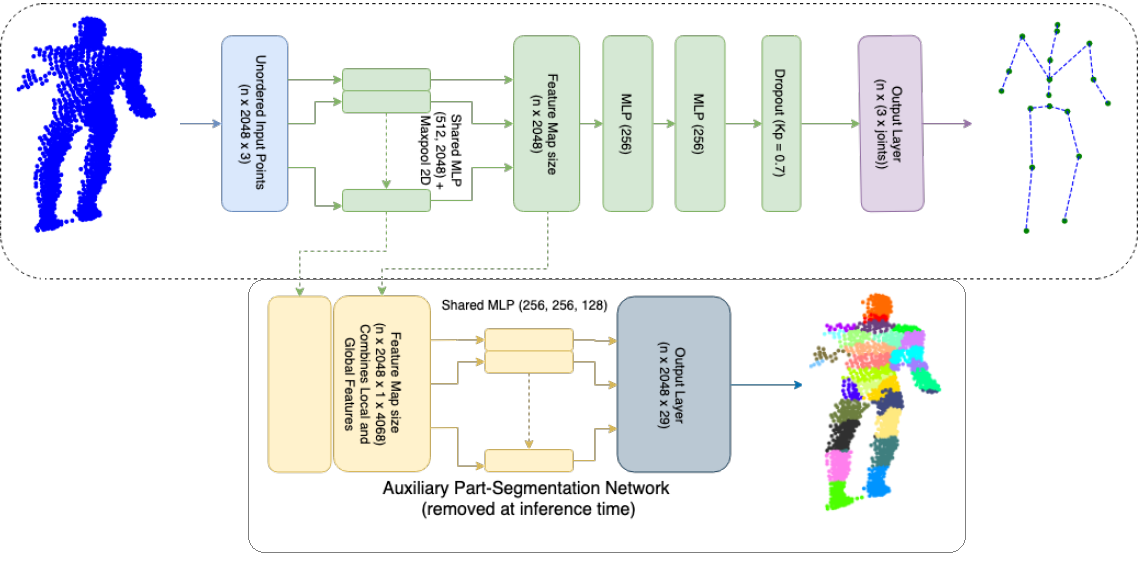
\includegraphics[height=200px]{images/related_work/pbpe2.PNG}
  \caption{The Point-Based Pose Estimation model architecture \cite{Ali19}.}
  \label{fig:PBPE}
\end{center}
\end{figure}

\noindent
As already mentioned, the unorganized and irregular depth input represented by a point cloud is a key factor in this architecture. For this very reason, the engagement of the classic convolution operation would be meaningless, since the point cloud has provides no explicit spatial information about the neighboring points. In this case, pseudo-convolutions with a kernel size of $1\times1$ are employed. The point of such pseudo-convolution layers is a reduction (or expansion) of dimensionality in the filter space. % TODO najst definicie a popis z prezentacie

% According to our experiments, without the segmentation sub-network, the model tends to slightly overfit the train data. The loss of the auxiliary segmentation branch is engaged with weight \textit{w=0.01} to help the model generalize better on previously unseen data.




\subsection{Data pre-processing}
% TODO marge datasets into one subsection ? - or at least the shared part of preprocessing (subsampling, segmentation)

\subsubsection{ITOP}

% ..TODO text + ref. Fig. \ref{fig:itop_seg} 

\begin{figure}[H]
\begin{center}
  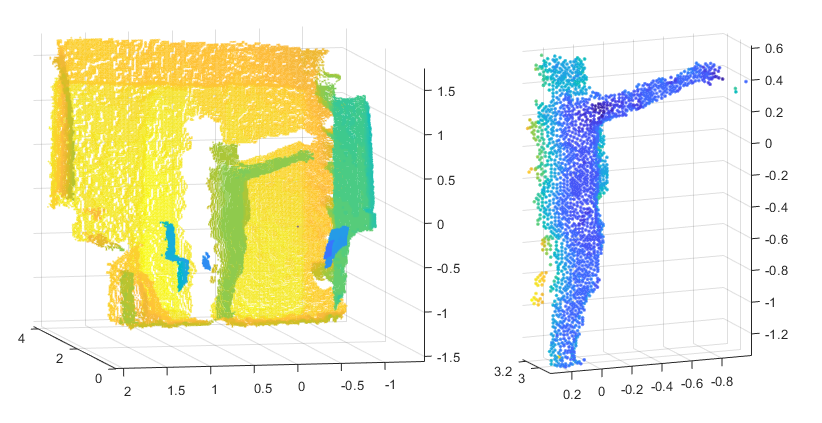
\includegraphics[height=140px]{images/implementation/itop_seg.png}
  \caption[Sample point cloud from ITOP-front dataset \cite{haque2016viewpoint}.]{ Sample point cloud from ITOP-front dataset \cite{haque2016viewpoint}, left – before, right – after segmentation.}
  \label{fig:itop_seg}
\end{center}
\end{figure}

\subsubsection{UBC3V}

Depending on the single or multi-view approach, the input point clouds are treated each as a single sample, or the different viewpoints of the same frame are merged into a single point cloud. In case of the UBC3V dataset, samples from three cameras are merged together. % TODO vysvetlit preco, .. obsahuje pomerne zlozite pozy
\par
\vspace{5mm}
\noindent
As the next pre-processing step, the point clouds were subsampled to the specified number of points (2048 points in our case) using the farthest point sampling technique. The input point clouds and the corresponding joint locations were normalized to the range [-1, 1] using the minimum and maximum values of the whole training set. Concerning the validation and test data, there were two options, how to normalize them – either using the scaling parameters of the training set, or scale the validation and test set to the specified range (with its own parameters). However, since the model is designed to work in real-time, the test data will most likely be fed into the network one-by-one, in which case, the only possible option is scaling using the parameters of the train set.\par
%\vspace{5mm}
%\noindent
%In order to increase the number of joints in the skeletal model, in some of the experiments, the interpolation of the joint locations was performed as another part of the pre-processing pipeline.  \textcolor{red}{TODO compare 29 vs 35 joints in Table ..} It is interesting to observe how the number of joints in the skeleton (and the complexity of the model) influences the pose estimation results.

\subsubsection{MHAD}
% TODO rozpisat podrobnejsie ?
The MHAD dataset provides each frame captured from two camera viewpoints, one situated in the front, the other one in the back of the subject.
Based on existing studies, inference from multi-view input data is expected to give more accurate results, however the single-view based estimation is far more useful in most of the real-time applications. Therefore, we have carried out experiments inferring from multi-view, as well as single-view input data.\par
\vspace{5mm}

\begin{figure}[H]
\begin{center}
  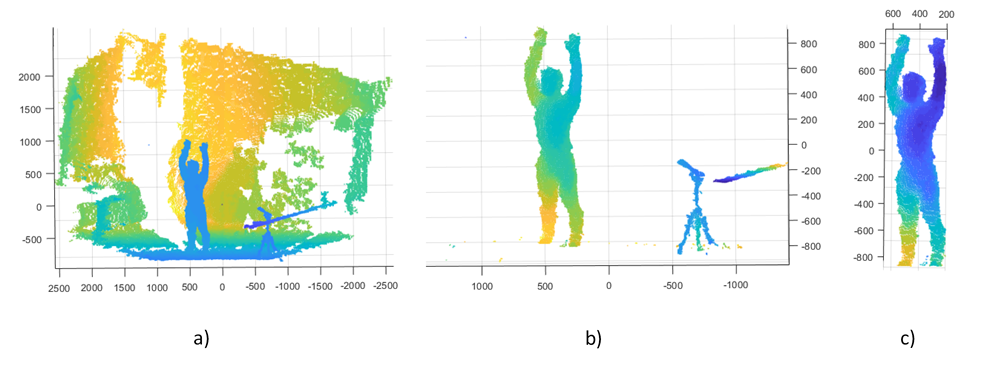
\includegraphics[height=140px]{images/implementation/mhad.png}
  \caption[Sample point cloud from MHAD dataset \cite{Vidal:2013:BMC:2478277.2478412}.]{ Sample point cloud from MHAD dataset \cite{Vidal:2013:BMC:2478277.2478412} a) before segmentation, b) after removing the background and floor, c) after final clustering.}
  \label{fig:mhad}
\end{center}
\end{figure}

\noindent
Since this dataset captures real-world data, the depth data contain a lot of noise. Therefore, we consider suitable preprocessing as a very important step. First, the background wall and ground floor are removed by MSAC plane fitting (which is a variation of RANSAC algorithm). Then, the segmentation of the point cloud into clusters based on Euclidean distance is used, and the biggest cluster is considered the desired subject. Fig. \ref{fig:mhad} depicts a sample from MHAD dataset, before and after applying the segmentation pipeline.\par

\vspace{5mm}
\noindent
The stated dataset does not provide any partition into train and test data. Thus, the test data was selected as randomly sampled 25\% of the whole dataset during the experiments, while the rest was marked as the train set.\par
\vspace{5mm}
\noindent 
As already pointed out in the original proposal of the PBPE model, the skeleton representation in the MHAD dataset is very detailed, yielding a total of 35 skeletal joints. Though this provides the ability of estimating the pose with higher complexity, some of the joints have the locations in the skeleton representation so close to each other, they may be considered redundant when estimating a full-body pose. Among these joints are two pairs of nodes located at toe tips and one additional pair of nodes representing the fingertips.
\textcolor{red}{TODO compare 29 vs 35 joints in Table - in Results chapter} As shown in Table ..., it is interesting to observe how the number of joints in the skeleton (and the complexity of the model) influences the pose estimation results.


 \section{Four-channel Pose Estimation}

\vspace{5mm}
\begin{figure}[H]
\begin{center}
  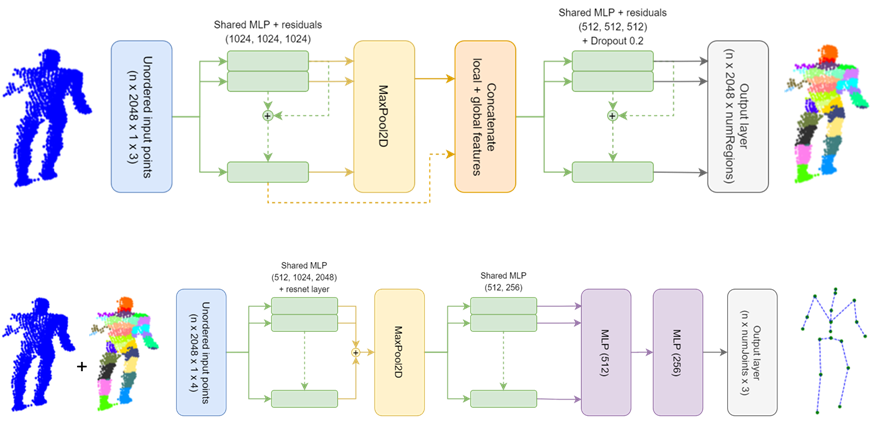
\includegraphics[width=\textwidth]{images/implementation/4chan_pipeline.png}
  \caption[The Four-channel Pose Estimation pipeline.]{ The Four-channel Pose Estimation pipeline: First, point clouds are segmented into body regions in the segmentation network (up), then the input point clouds are concatenated with the predicted body regions as a fourth channel, and are fed into the regression network (down).}
  \label{fig:4chan_pipeline}
\end{center}
\end{figure}


